\section{Future work: integration of DVMS with OpenStack}
\label{sec:future_work}

\subsection{DVMS: a dynamic scheduler for virtual machines}

% \begin{itemize}

% 	\item Dynamic scheduler for virtual machines.

% 	\item Leverage a locality aware p2p overlay.

% 	\item Successfuly tested in simulator (simgrid) and computing grid (grid'5000).

% \end{itemize}

DVMS \cite{quesnel:ispa2013} (Distributed Virtual Machine 
Scheduler) is a framework that schedules VMs cooperatively and dynamically in
large scale distributed systems, following a ring topology. When one of the DVMS
agents cannot guarantee needs of its hosted VMs it starts an iterative 
scheduling procedure~(ISP), becoming thus the initiator of the ISP.

The ISP is forwarded to the next free agent, which will attempt to find a viable
mapping. The last step is repeated until the ISP succeeds. When a viable mapping
has been found, the last peer (leader) reconfigures the system by performing 
adequate VM migrations. Proof has been made that if a solution exits, it will
always be found, and experiments have shown that in most cases ISPs involve 
only few nodes. Moreover, several ISPs can occur independently:
scheduling is performed on partitions of the system that are created dynamically
, which significantly improves reactivity of the system.


\subsection{Integration of DVMS in OpenStack}

\label{sub:sec:integration_dvms}

\begin{itemize}

\item We propose to replace "nova-scheduler" (static scheduler) by DVMS.

\begin{figure}[h]
	\centering
	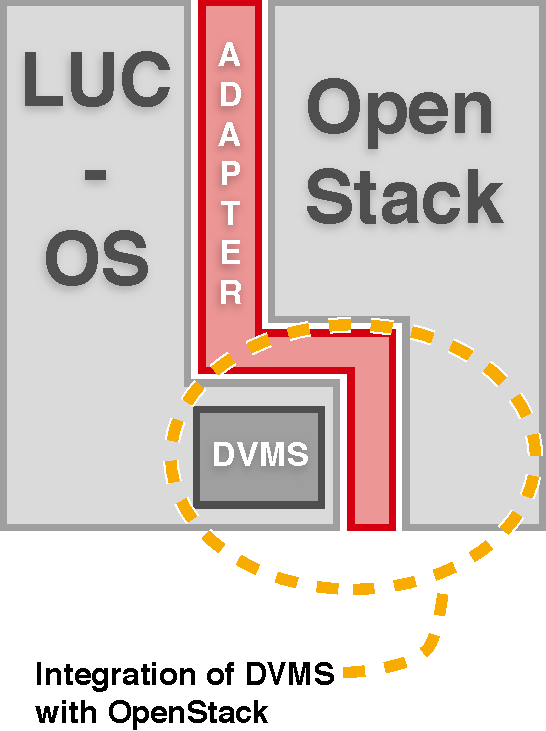
\includegraphics[width=0.50\linewidth]{Figures/dvms_openstack.pdf}
	\caption{Integration of DVMS in OpenStack.}%
	\label{fig:integration}%
	%\vspace*{-.8cm}
\end{figure}

% \item Use of an "Adapter" object that will wrap DVMS and integrate well with OpenStack, as described in figure \ref{fig:integration}
% 	\begin{itemize}
% 		\item It will consume messages that are destinated to "nova-scheduler"

% 		\item Each message will be converted to a "Dvms" message.

% 		\item Each message produced by Dvms will be converted to an OpenStack message and added to the Queue.

% 	\end{itemize}

Considering the fact that nova-scheduler currently performs static scheduling, 
as introduced in section \ref{sub:sec:revisiting_openstack}, we decided to 
replace it by DVMS. Before going more into technical details of the integration,
OpenStack's service architecture is flexible: service follow the "shared nothing
memory" principle and communicate through an AMQP bus. This means that each 
service follows a "protocol" : when it consumes all received message, in return
it execute an action and produces a specific messsage. 

With this in mind, we depicted in figure \ref{fig:integration} the way we want 
to integrate DVMS with OpenStack: we use an adapter object that consumes 
messages that are destinated to nova-scheduler, forward it to DVMS and translate
messages produced by DMVS in message from the nova-scheduler protocol. We think
that this method will minimize modification on Nova service.

\end{itemize}